

% microtype: Tipografía.
% mathpazo: Usa la fuente Palatino.
\documentclass[a4paper, 11pt]{article}
\usepackage[protrusion=true,expansion=true]{microtype}
\usepackage{mathpazo}
\usepackage{booktabs}
\usepackage{multicol}
\usepackage{multirow}

% Indentación de párrafos para Palatino
\setlength{\parindent}{0pt}
  \parskip=8pt
\linespread{1.05} % Change line spacing here, Palatino benefits from a slight increase by default


%%% Castellano.
% noquoting: Permite uso de comillas no españolas.
% lcroman: Permite la enumeración con numerales romanos en minúscula.
% fontenc: Usa la fuente completa para que pueda copiarse correctamente del pdf.
\usepackage[spanish,es-noquoting,es-lcroman]{babel}
\usepackage[utf8]{inputenc}
\usepackage[T1]{fontenc}
\selectlanguage{spanish}


%%% Gráficos
\usepackage{graphicx} % Required for including pictures
\usepackage{wrapfig} % Allows in-line images
\usepackage[usenames,dvipsnames]{color} % Coloring code


%%% Matemáticas
\usepackage{amsmath}
\usepackage[hidelinks]{hyperref}
%%% Código


\usepackage{listings}
\usepackage{graphicx}

%% Listing settings

\usepackage{color}

\definecolor{dkgreen}{rgb}{0,0.6,0}
\definecolor{gray}{rgb}{0.5,0.5,0.5}
\definecolor{mauve}{rgb}{0.58,0,0.82}

\lstset{frame=tb,
  language=Java,
  aboveskip=3mm,
  belowskip=3mm,
  showstringspaces=false,
  columns=flexible,
  basicstyle={\small\ttfamily},
  numbers=none,
  numberstyle=\tiny\color{gray},
  keywordstyle=\color{blue},
  commentstyle=\color{dkgreen},
  stringstyle=\color{mauve},
  breaklines=true,
  breakatwhitespace=true,
  tabsize=3
}



%%% Bibliografía
\makeatletter
\renewcommand\@biblabel[1]{\textbf{#1.}} % Change the square brackets for each bibliography item from '[1]' to '1.'
\renewcommand{\@listI}{\itemsep=0pt} % Reduce the space between items in the itemize and enumerate environments and the bibliography



%----------------------------------------------------------------------------------------
%	TÍTULO
%----------------------------------------------------------------------------------------
% Configuraciones para el título.
% El título no debe editarse aquí.
\renewcommand{\maketitle}{
  \begin{flushright} % Right align
  
  {\LARGE\@title} % Increase the font size of the title
  
  \vspace{50pt} % Some vertical space between the title and author name
  
  {\large\@author} % Author name
  \\\@date % Date
  \vspace{40pt} % Some vertical space between the author block and abstract
  \end{flushright}
}

%% Título
\title{\textbf{Memoria de la práctica 4}\\ % Title
Algorítmica} % Subtitle

\author{\textsc{Fco. Javier Sáez Maldonado}\\ % Author
\textsc{Laura Gómez Garrido}\\
\textsc{Luis Antonio Ortega Andrés}\\
\textsc{Pedro Bonilla Nadal}\\
\textsc{Daniel Pozo Escalona}\vspace{2cm}
\\{\textit{Universidad de Granada}}} % Institution

\date{\today} % Date



%----------------------------------------------------------------------------------------
%	DOCUMENTO
%----------------------------------------------------------------------------------------

\begin{document}

\maketitle % Print the title section


%% Índice
{\parskip=2pt
  \tableofcontents
}
\pagebreak

%%% Inicio del documento


\section{Problema}
 Referencia: El puzzle “\textbf{La Maleta de Luke}” (El Profesor Layton y la Caja de
Pandora, Nintendo DS).


Diversos videojuegos de la categoría puzzle ofrecen rompecabezas que pueden
ser estudiados como un problema de exploración en grafos. En particular, el puzzle “La maleta de Luke” presentado en El profesor Layton y la Caja de Pandora para Nintendo DS, supone que hay una maleta y diversos objetos que tenemos que introducir en ella
sin que se solapen, cada uno de unas dimensiones determinadas.
Estos problemas se pueden discretizar, de modo que en nuestro caso dividiremos
la maleta en un rectángulo de 6 casillas de alto por 9 de ancho, y cada objeto también lo
discretizaremos con estas mismas dimensiones:\\
\begin{center}
	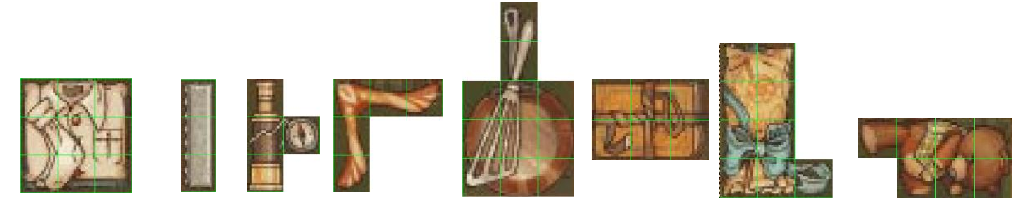
\includegraphics[scale=0.35]{piezas.png}
\end{center}

Cada pieza, a la hora de colocarla en una posición de la maleta, puede
rotarse 0º, 90º, 180º o 270º para alcanzar la solución. De este modo, el
puzzle se resuelve colocando las piezas según la siguiente figura:
\begin{center}
	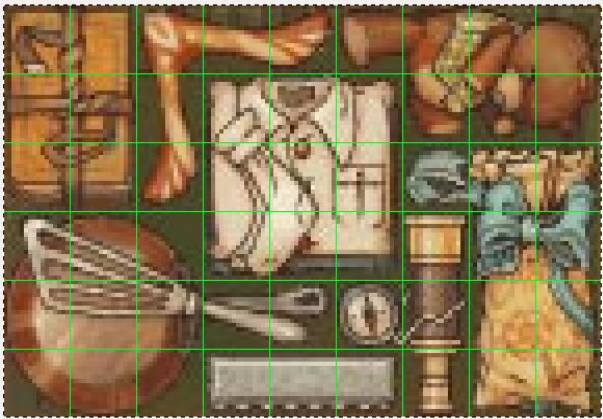
\includegraphics[scale=0.35]{solucion.png}
\end{center}


Se pide diseñar e implementar un algoritmo de exploración en grafos
(BackTracking o Branch\&Bound) que solucione este problema con el tamaño de maleta
y piezas descritas en este apartado.

\section{Solución}




\subsubsection{La complejidad del algoritmo}


\subsubsection{Eficiencia práctica}

\subsubsection{Eficiencia híbrida}

\section{Conclusión}





Se debe 
incluir un análisis del problema
.
2.
Escoger  una  técnica  (BackTracking  o  Branch\&Bound)  y  justificar  s
u  elección 
frente a la otra metodología no seleccionada.
3.
Diseño  de  la  solución,  describiendo  cada  una  de  las  componentes  de  la  misma 
relacionándola   con   las   componentes   de   un   algoritmo 
BackTracking   o 
Branch\&Bound, según la técnica escogida
.
4.
Esqueleto  del  al
goritmo  (pseudocódigo)  que  soluciona  el  problema,  explicando 
cómo  se  ha  incorporado  cada  una  de  las  componentes 
de  diseño  de  la  técnica 
(BackTracking o Branch\&Bound, según se aplique)
.
5.
Explicación   del   funcionamiento   del   algoritmo,   sobre   un   caso   de   ejemplo 
pequeño propuesto por los estudiantes.

 
6.
Enunciado  de  un  problema  o  caso  real  donde  se  pueda  utilizar 
la  técnica 
seleccionada
para solucionarlo (distinto de los comentados en clase).
7.
Cálculo del orden de eficiencia teórico del algoritmo.
8.
Instrucciones sobre 
cómo compilar y ejecutar el código de l
\end{document}
